% NE 630 -- Lesson 19 OpenMC unit-cell modeling cheat sheet
% Standalone source: latexmk -xelatex -interaction=nonstopmode -halt-on-error lesson_19_handout.tex
% NE 630 -- shared reading-guide definitions, Lessons 15--21
% Included by lesson_15_handout.tex through lesson_21_handout.tex.
% Layout/palette adapted from the user's ne630boardhandout class.
% Content: supplied chapter(1).tex and lecture_15.tex through lecture_19.tex.
% The supplied chapter numbers the four-factor discussion as Section 4.5.
% Drawings below adapt supplied Fig. 4.1, Fig. 4.5, Fig. 4.6, and the L19
% pin-cell drawing. They are qualitative schematics, not simulation results.
\documentclass[10pt,letterpaper]{article}
\usepackage{amsmath,mathtools}
\usepackage{libertinus,microtype}
\usepackage[left=0.48in,right=0.48in,top=0.48in,bottom=0.44in,
  headheight=20pt,headsep=5pt,footskip=17pt,includeheadfoot]{geometry}
\usepackage{graphicx,xcolor,tabularx,booktabs,array,ragged2e}
\usepackage{tikz}
\usetikzlibrary{arrows.meta,calc,positioning,patterns}
\usepackage[most]{tcolorbox}
\usepackage{fancyhdr,lastpage}
\usepackage[hidelinks]{hyperref}
\hypersetup{pdfauthor={NE 630},pdfsubject={The Power Reactor Core}}
\definecolor{KSUPurple}{HTML}{512888}
\definecolor{KSUDeepPurple}{HTML}{3B1B64}
\definecolor{KSUOrange}{HTML}{CA7C1B}
\definecolor{KSUGray}{HTML}{5D5D5D}
\setlength{\parindent}{0pt}
\setlength{\parskip}{3pt}
\setlength{\emergencystretch}{1.5em}
\setlength{\abovedisplayskip}{4pt}
\setlength{\belowdisplayskip}{4pt}
\setlength{\abovedisplayshortskip}{2pt}
\setlength{\belowdisplayshortskip}{3pt}
\setlength{\jot}{3pt}
\renewcommand{\arraystretch}{1.12}
\newcolumntype{Y}{>{\RaggedRight\arraybackslash}X}
\newcommand{\LessonNo}{15}
\pagestyle{fancy}
\fancyhf{}
\fancyhead[L]{\sffamily\bfseries\small NE 630}
\fancyhead[C]{\sffamily\small The Power Reactor Core}
\fancyhead[R]{\sffamily\bfseries\small Lesson \LessonNo}
\fancyfoot[L]{\sffamily\scriptsize  }
\fancyfoot[C]{\sffamily\scriptsize \thepage\ of \pageref*{LastPage}}
\fancyfoot[R]{\sffamily\scriptsize }
\renewcommand{\headrulewidth}{0.5pt}
\makeatletter
\renewcommand{\headrule}{\hbox to\headwidth{\color{KSUPurple}\leaders\hrule height .5pt\hfill}}
\makeatother
\newcommand{\Lesson}[4]{%
  \renewcommand{\LessonNo}{#1}%
  \noindent\begin{minipage}[c]{0.025\linewidth}\color{KSUPurple}\rule{3.5pt}{32pt}\end{minipage}%
  \begin{minipage}[c]{0.815\linewidth}
   {\sffamily\bfseries\fontsize{18}{20}\selectfont #2}\par
   {\sffamily\fontsize{9}{10.5}\selectfont #4}
  \end{minipage}\hfill
  \begin{minipage}[c]{0.14\linewidth}\raggedleft
    {\sffamily\color{KSUPurple}\bfseries\fontsize{25}{26}\selectfont #1}\par
    {\sffamily\scriptsize LESSON}
  \end{minipage}\par\vspace{3pt}
  \begin{tcolorbox}[enhanced,boxrule=.45pt,arc=1pt,colback=KSUPurple!4,
   colframe=KSUPurple!40,left=5pt,right=5pt,top=3pt,bottom=3pt,
   before skip=0pt,after skip=6pt]
   \sffamily\fontsize{9}{10.5}\selectfont\textbf{Read:} #3
  \end{tcolorbox}}
\newcommand{\Sec}[2]{\par\addvspace{5pt}\noindent
  \colorbox{KSUPurple}{\color{white}\sffamily\bfseries\fontsize{9}{10}\selectfont\strut #1}
  \hspace{3pt}{\sffamily\bfseries\color{KSUDeepPurple}\fontsize{10.2}{11.5}\selectfont #2}\par\vspace{1pt}}
\newcommand{\eqread}[1]{{\sffamily\fontsize{7.9}{9}\selectfont\color{KSUGray}#1}}
\newcommand{\figcap}[1]{\par\vspace{1pt}{\sffamily\fontsize{7.7}{9}\selectfont\color{KSUGray}#1}\par}
\newtcolorbox{KeyBox}[1]{enhanced,boxrule=.45pt,arc=1pt,
 colback=KSUPurple!3,colframe=KSUPurple!40,left=5pt,right=5pt,top=4pt,bottom=4pt,
 before skip=4pt,after skip=4pt,before upper=\RaggedRight,fonttitle=\sffamily\bfseries\small,
 coltitle=KSUDeepPurple,title={#1},colbacktitle=KSUPurple!7,
 titlerule=0pt,toptitle=2pt,bottomtitle=2pt}
\newtcolorbox{Explore}[1]{enhanced,boxrule=.5pt,arc=1pt,
 colback=KSUOrange!5,colframe=KSUOrange!65,left=6pt,right=6pt,top=4pt,bottom=4pt,
 before skip=7pt,after skip=3pt,before upper=\RaggedRight,
 title={OpenMC \enspace\textbar\enspace #1},fonttitle=\sffamily\bfseries\fontsize{9}{10}\selectfont,
 coltitle=KSUDeepPurple,colbacktitle=KSUOrange!10,titlerule=0pt,toptitle=2pt,bottomtitle=2pt}
\newcommand{\SourceLine}[1]{\par\vspace{2pt}{\sffamily\fontsize{7.2}{8.4}\selectfont\color{KSUGray}#1}\par}
\newcommand{\colstart}{\begin{minipage}[t]{.482\linewidth}\vspace{0pt}\RaggedRight}
\newcommand{\colnext}{\end{minipage}\hfill\begin{minipage}[t]{.482\linewidth}\vspace{0pt}\RaggedRight}
\newcommand{\colend}{\end{minipage}\par}
\newcommand{\uunit}[1]{\,\mathrm{#1}}
\newcommand{\metal}{\mathrm{metal}}
\newcommand{\water}{\mathrm{w}}
\newcommand{\fiiso}{\mathrm{fi}}
\newcommand{\feiso}{\mathrm{fe}}
\newcommand{\nucl}[2]{\ensuremath{{}^{#1}\mathrm{#2}}}



% Five reactor motifs, adapted from the supplied Fig. 4.1, with a compact TRISO zoom.
\newcommand{\FamilyFigure}{%
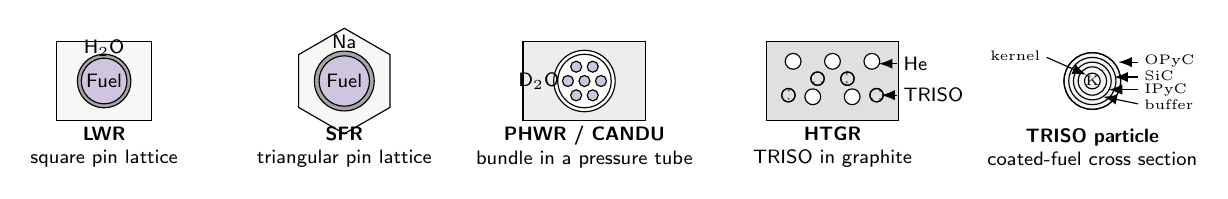
\begin{tikzpicture}[x=1cm,y=1cm,line width=.42pt,font=\sffamily\fontsize{7.5}{8.5}\selectfont,
 every node/.style={inner sep=1pt},>=Latex]
\begin{scope}[shift={(0,0)}]
 \draw[fill=black!3] (-.60,-.50) rectangle (.60,.50);
 \draw[fill=black!35] (0,0) circle (.34);
 \draw[fill=KSUPurple!27] (0,0) circle (.29);
 \node at (0,0) {Fuel}; \node at (0,.42) {H$_2$O};
 \node[align=center] at (0,-.84) {\textbf{LWR}\\square pin lattice};
\end{scope}
\begin{scope}[shift={(3.05,0)}]
 \draw[fill=black!3] (90:.67)--(30:.67)--(-30:.67)--(-90:.67)--(-150:.67)--(150:.67)--cycle;
 \draw[fill=black!35] (0,0) circle (.38);
 \draw[fill=KSUPurple!27] (0,0) circle (.32);
 \node at (0,0) {Fuel}; \node at (0,.50) {Na};
 \node[align=center] at (0,-.84) {\textbf{SFR}\\triangular pin lattice};
\end{scope}
\begin{scope}[shift={(6.10,0)}]
 \draw[fill=black!7] (-.78,-.50) rectangle (.78,.50);
 \draw[fill=white] (0,0) circle (.39);
 \draw (0,0) circle (.34);
 \foreach \ang in {0,60,...,300}{\draw[fill=KSUPurple!27] (\ang:.21) circle (.07);} 
 \draw[fill=KSUPurple!27] (0,0) circle (.07);
 \node[align=center] at (-.58,0) {D$_2$O};
 \node[align=center] at (0,-.84) {\textbf{PHWR / CANDU}\\bundle in a pressure tube};
\end{scope}
\begin{scope}[shift={(9.25,0)}]
 \draw[fill=black!12] (-.84,-.50) rectangle (.84,.50);
 \foreach \x/\y in {-.50/.25,0/.25,.50/.25,-.25/-.20,.25/-.20}{\draw[fill=white] (\x,\y) circle (.10);} 
 \foreach \x/\y in {-.56/-.18,-.19/.03,.19/.03,.56/-.18}{
   \draw[fill=KSUPurple!10,pattern=dots,pattern color=KSUPurple!70] (\x,\y) circle (.085);
   \draw (\x,\y) circle (.085);
 }
 \node[anchor=west] at (.86,.22) {He};
 \draw[->] (.82,.22)--(.59,.22);
 \node[anchor=west] at (.86,-.18) {TRISO};
 \draw[->] (.82,-.18)--(.62,-.18);
 \node[align=center] at (0,-.84) {\textbf{HTGR}\\TRISO in graphite};
\end{scope}
\begin{scope}[shift={(12.55,0)}]
 \draw[fill=KSUPurple!70] (0,0) circle (.10);  % kernel
 \draw[fill=KSUPurple!18] (0,0) circle (.18);  % buffer
 \draw[fill=gray!25] (0,0) circle (.24);       % inner PyC
 \draw[fill=green!12!black!8] (0,0) circle (.30); % SiC
 \draw[fill=gray!8] (0,0) circle (.36);        % outer PyC
 \foreach \r in {.10,.18,.24,.30,.36}{\draw (0,0) circle (\r);} 
 \node[font=\tiny] at (0,0) {K};
 \node[font=\tiny,anchor=west] at (.62,.25) {OPyC}; \draw[->] (.58,.24)--(.33,.24);
 \node[font=\tiny,anchor=west] at (.62,.06) {SiC};  \draw[->] (.58,.05)--(.28,.05);
 \node[font=\tiny,anchor=west] at (.62,-.12) {IPyC};\draw[->] (.58,-.11)--(.21,-.11);
 \node[font=\tiny,anchor=west] at (.62,-.30) {buffer};\draw[->] (.58,-.29)--(.14,-.20);
 \node[font=\tiny,anchor=east] at (-.62,.32) {kernel};\draw[->] (-.58,.30)--(-.08,.08);
 \node[align=center] at (0,-.84) {\textbf{TRISO particle}\\coated-fuel cross section};
\end{scope}
\end{tikzpicture}}

% Square and hexagonal pin cells, adapted from the L19 cell figure and Fig. 4.1.
\newcommand{\PinCellsFigure}{%
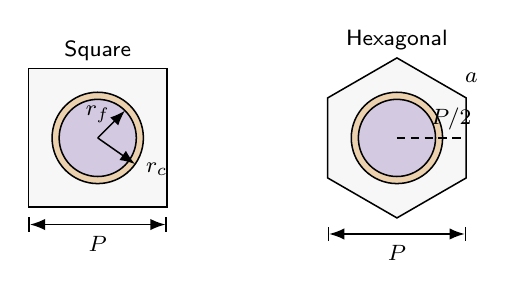
\begin{tikzpicture}[x=1cm,y=1cm,font=\sffamily\fontsize{8.5}{10}\selectfont,
 line width=.55pt,>=Latex,every node/.style={inner sep=1pt}]
\begin{scope}[shift={(0,0)}]
 \draw[fill=black!3] (-.88,-.88) rectangle (.88,.88);
 \draw[fill=KSUOrange!35] (0,0) circle (.58);
 \draw[fill=KSUPurple!25] (0,0) circle (.49);
 \draw[->] (0,0)--(45:.49) node[midway,above left=-1pt] {$r_f$};
 \draw[->] (0,0)--(-35:.58);\node[anchor=west] at (.57,-.40) {$r_c$};
 \draw[|<->|] (-.88,-1.10)--(.88,-1.10) node[midway,below=3pt] {$P$};
 \node at (0,1.10) {Square};
\end{scope}
\begin{scope}[shift={(3.80,0)}]
 \draw[fill=black!3] (90:1.016)--(30:1.016)--(-30:1.016)--(-90:1.016)--(-150:1.016)--(150:1.016)--cycle;
 \draw[fill=KSUOrange!35] (0,0) circle (.58);
 \draw[fill=KSUPurple!25] (0,0) circle (.49);
 \draw[densely dashed] (0,0)--(.88,0);
 \node[above] at (.69,.05) {$P/2$};
 \draw[|<->|] (-.88,-1.22)--(.88,-1.22) node[midway,below=3pt] {$P$};
 \node at (0,1.24) {Hexagonal};
 \node[anchor=west] at (.82,.77) {$a$};
\end{scope}
\end{tikzpicture}}

% Bookkeeping cycle adapted from supplied Fig. 4.5 (not a spatial plot).
\newcommand{\CycleFigure}{%
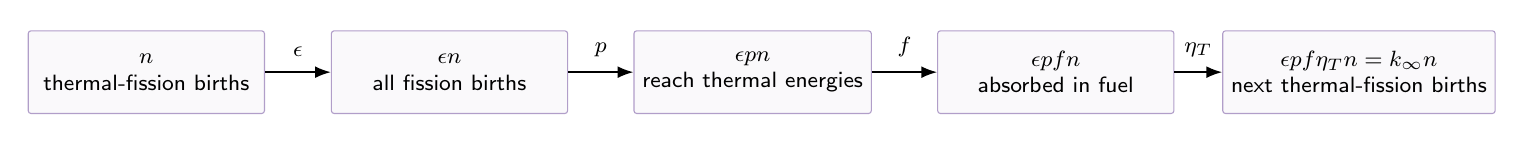
\begin{tikzpicture}[x=1cm,y=1cm,>=Latex,
 box/.style={draw=KSUPurple!45,fill=KSUPurple!3,rounded corners=1pt,
 minimum width=3.0cm,minimum height=1.05cm,align=center,inner sep=3pt},
 every node/.style={font=\sffamily\fontsize{8.2}{9.5}\selectfont}]
 \node[box] (n) at (0,0) {$n$\\thermal-fission births};
 \node[box] (en) at (3.85,0) {$\epsilon n$\\all fission births};
 \node[box] (epn) at (7.7,0) {$\epsilon p n$\\reach thermal energies};
 \node[box] (epfn) at (11.55,0) {$\epsilon p f n$\\absorbed in fuel};
 \node[box] (kn) at (15.4,0) {$\epsilon p f\eta_T n=k_\infty n$\\next thermal-fission births};
 \draw[->,line width=.6pt] (n)--(en) node[midway,above=2pt] {$\epsilon$};
 \draw[->,line width=.6pt] (en)--(epn) node[midway,above=2pt] {$p$};
 \draw[->,line width=.6pt] (epn)--(epfn) node[midway,above=2pt] {$f$};
 \draw[->,line width=.6pt] (epfn)--(kn) node[midway,above=2pt] {$\eta_T$};
\end{tikzpicture}}

% Qualitative Doppler/space-energy shielding sketch, adapted from Fig. 4.6.
\newcommand{\ResonanceFigure}{%
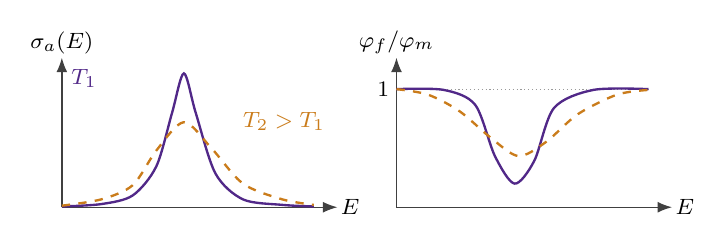
\begin{tikzpicture}[x=1cm,y=1cm,>=Latex,
 ax/.style={->,line width=.5pt,draw=black!75},
 cold/.style={line width=.85pt,draw=KSUPurple},
 hot/.style={line width=.85pt,draw=KSUOrange,dashed},
 every node/.style={font=\sffamily\fontsize{8.1}{9}\selectfont,inner sep=1pt}]
\begin{scope}
 \draw[ax] (0,0)--(3.5,0) node[right] {$E$};
 \draw[ax] (0,0)--(0,1.9) node[above] {$\sigma_a(E)$};
 \draw[cold] plot[smooth] coordinates {(0,.01)(.5,.04)(.9,.15)(1.2,.52)(1.4,1.2)(1.55,1.7)(1.7,1.2)(1.95,.43)(2.3,.10)(2.8,.03)(3.2,.01)};
 \draw[hot] plot[smooth] coordinates {(0,.02)(.5,.10)(.9,.28)(1.2,.72)(1.55,1.08)(1.9,.75)(2.3,.30)(2.8,.10)(3.2,.03)};
 \node[anchor=west,text=KSUPurple] at (.08,1.63) {$T_1$};
 \node[anchor=west,text=KSUOrange] at (2.26,1.09) {$T_2>T_1$};
\end{scope}
\begin{scope}[shift={(4.25,0)}]
 \draw[ax] (0,0)--(3.5,0) node[right] {$E$};
 \draw[ax] (0,0)--(0,1.9) node[above] {$\varphi_f/\varphi_m$};
 \draw[black!40,densely dotted] (0,1.5)--(3.2,1.5);
 \node[anchor=east] at (-.05,1.5) {$1$};
 \draw[cold] plot[smooth] coordinates {(0,1.5)(.6,1.49)(1,1.3)(1.25,.65)(1.5,.3)(1.75,.59)(2,1.26)(2.5,1.49)(3.2,1.5)};
 \draw[hot] plot[smooth] coordinates {(0,1.5)(.4,1.43)(.8,1.22)(1.2,.88)(1.55,.65)(1.9,.83)(2.3,1.18)(2.8,1.43)(3.2,1.49)};
\end{scope}
\end{tikzpicture}}

\usepackage{listings}
\hypersetup{pdftitle={NE 630: Lesson 19 -- OpenMC Unit-Cell Modeling Cheat Sheet}}

\lstdefinestyle{omc}{
  language=Python,
  basicstyle=\ttfamily\fontsize{6.65}{7.45}\selectfont,
  keywordstyle=\color{KSUDeepPurple}\bfseries,
  commentstyle=\color{KSUGray}\itshape,
  stringstyle=\color{KSUOrange!85!black},
  columns=fullflexible,keepspaces=true,showstringspaces=false,
  breaklines=true,breakatwhitespace=true,
  aboveskip=2pt,belowskip=2pt,
  frame=single,rulecolor=\color{KSUPurple!25},
  framesep=3pt,xleftmargin=1pt,xrightmargin=1pt
}
\lstset{style=omc}

\begin{document}
\fontsize{8.7}{10.25}\selectfont
\RaggedRight

\Lesson{19}{OpenMC unit-cell modeling: cheat sheet}
 {Condensed from the PWR and SFR unit-cell notebooks in Lessons 17 and 19.}
 {What is the minimum complete model for an infinite pin lattice?}

\begin{KeyBox}{The five pieces of an OpenMC model}
\textbf{Materials} $\rightarrow$ \textbf{surfaces/regions} $\rightarrow$ \textbf{cells/geometry}
$\rightarrow$ \textbf{settings} $\rightarrow$ \textbf{tallies}.  Bundle them in
\texttt{openmc.Model}, run in an isolated directory, and read the resulting statepoint.
Use reflective outer and axial boundaries for a no-leakage, infinite-lattice $k_\infty$ model.
Internal fuel/cladding surfaces remain transmitting (the default).
\end{KeyBox}

\colstart
\Sec{1}{Shared setup and dimensions}
\begin{lstlisting}
import os, tempfile
from pathlib import Path
import numpy as np
import openmc

xs = os.environ["OPENMC_CROSS_SECTIONS"]
openmc.config["cross_sections"] = xs

rf, rc, P, H = 0.45, 0.46, 1.20, 1.0 # cm
fuel_s = openmc.ZCylinder(r=rf)
clad_s = openmc.ZCylinder(r=rc)
z0 = openmc.ZPlane(z0=-H/2, boundary_type="reflective")
z1 = openmc.ZPlane(z0= H/2, boundary_type="reflective")
axial = +z0 & -z1
\end{lstlisting}
Always check $P>2r_c$.  Use one consistent axial height $H$ in the
geometry and volumes; $H=1$ cm is convenient.

\Sec{2}{PWR materials: square lattice}
\begin{lstlisting}
fuel = openmc.Material(name="UO2 fuel")
fuel.add_element("U", 1.0, enrichment=4.0) # wt% U-235
fuel.add_element("O", 2.0)
fuel.set_density("g/cm3", 10.5)
fuel.temperature = 1200.0

clad = openmc.Material(name="Zr cladding")
clad.add_element("Zr", 1.0)
clad.set_density("g/cm3", 6.6)

cool = openmc.model.borated_water(
    boron_ppm=800.0, temperature=600.0,
    pressure=15.5, temp_unit="K", press_unit="MPa")
\end{lstlisting}
\texttt{borated\_water} supplies H$_2$O composition and
\texttt{c\_H\_in\_H2O} thermal scattering.  Enrichment passed to
\texttt{add\_element} is weight percent.

\Sec{3}{PWR regions, cells, and volumes}
\begin{lstlisting}
x0 = openmc.XPlane(x0=-P/2, boundary_type="reflective")
x1 = openmc.XPlane(x0= P/2, boundary_type="reflective")
y0 = openmc.YPlane(y0=-P/2, boundary_type="reflective")
y1 = openmc.YPlane(y0= P/2, boundary_type="reflective")
outer = +x0 & -x1 & +y0 & -y1 & axial

cells = [
  openmc.Cell(name="fuel", fill=fuel,
              region=-fuel_s & outer),
  openmc.Cell(name="cladding", fill=clad,
              region=+fuel_s & -clad_s & outer),
  openmc.Cell(name="coolant", fill=cool,
              region=+clad_s & outer)]
V = np.array([np.pi*rf**2,
              np.pi*(rc**2-rf**2),
              P**2-np.pi*rc**2])*H
for c, v in zip(cells, V): c.volume = float(v)
\end{lstlisting}
\colnext
\Sec{4}{SFR materials: explicit enrichment basis}
\begin{lstlisting}
e = 0.15  # U-235 atom fraction among uranium atoms
fuel = openmc.Material(name="UO2 fuel")
fuel.add_nuclide("U235", e)
fuel.add_nuclide("U238", 1.0-e)
fuel.add_element("O", 2.0)
fuel.set_density("g/cm3", 10.5)

clad = openmc.Material(name="steel cladding")
clad.add_element("Fe", 1.0)       # shortened example
clad.set_density("g/cm3", 7.13)

cool = openmc.Material(name="sodium coolant")
cool.add_nuclide("Na23", 1.0)
cool.set_density("g/cm3", 0.837)
\end{lstlisting}
For a specified alloy, replace the shortened Fe material by its full
elemental composition.  Adding U-235 and U-238 explicitly makes $e$ an
\emph{atom fraction}; do not confuse it with the weight-percent shortcut
used in the PWR example.

\Sec{5}{SFR regions: hexagonal lattice}
Here $P$ is the nearest-neighbor pitch (the hexagon's across-flats
dimension), so the hexagon side length is $P/\sqrt3$.
\begin{lstlisting}
hex_s = openmc.model.HexagonalPrism(
    edge_length=P/np.sqrt(3.0), orientation="x",
    boundary_type="reflective")
outer = -hex_s & axial

cells = [
  openmc.Cell(name="fuel", fill=fuel,
              region=-fuel_s & outer),
  openmc.Cell(name="cladding", fill=clad,
              region=+fuel_s & -clad_s & outer),
  openmc.Cell(name="coolant", fill=cool,
              region=+clad_s & outer)]
Ahex = np.sqrt(3.0)*P**2/2.0
V = np.array([np.pi*rf**2,
              np.pi*(rc**2-rf**2),
              Ahex-np.pi*rc**2])*H
for c, v in zip(cells, V): c.volume = float(v)
\end{lstlisting}

\begin{KeyBox}{Geometry sanity checks}
\vspace{-2pt}
\[
 \sum_rV_r=A_{\rm cell}H,\qquad
 A_{\rm sq}=P^2,\qquad A_{\rm hex}=\frac{\sqrt3}{2}P^2.
\]
Use \texttt{model.plot()} to inspect the geometry before spending histories.
Overlaps, gaps, a missing outer boundary, and a wrong hexagon side length
are the most expensive ``small'' mistakes.
\end{KeyBox}
\colend

\newpage
\Lesson{19}{OpenMC unit-cell modeling: run and reduce}
 {Use after defining \texttt{cells} and \texttt{V} on page 1.}
 {How do geometry and materials become defensible physical results?}

\colstart
\Sec{6}{Eigenvalue settings}
\begin{lstlisting}
settings = openmc.Settings(run_mode="eigenvalue")
settings.batches, settings.inactive = 60, 10
settings.particles, settings.seed = 2000, 19001
settings.source = openmc.IndependentSource(
    space=openmc.stats.Point((0., 0., 0.)),
    angle=openmc.stats.Isotropic(),
    energy=openmc.stats.Watt())
settings.temperature = {"method": "interpolation"}
\end{lstlisting}
Inactive batches converge the fission source; active batches estimate
responses.  Increase histories until uncertainty is small relative to the
difference you want to interpret.  A random seed aids reproducibility; an
independent seed is appropriate for a confirmation calculation.

\Sec{7}{Tallies: filter first, then score}
\begin{lstlisting}
cell_filter = openmc.CellFilter(cells)

# PWR groups: thermal, intermediate, fast [eV]
edges = [1.0e-5, 1.0, 1.0e5, 2.0e7]
rates = openmc.Tally(name="regional rates")
rates.filters = [cell_filter, openmc.EnergyFilter(edges)]
rates.scores = ["flux", "absorption", "nu-fission"]

# Optional fine spectrum, logarithmic in energy
E = np.geomspace(1.0e-5, 2.0e7, 161)
spec = openmc.Tally(name="regional spectrum")
spec.filters = [cell_filter, openmc.EnergyFilter(E)]
spec.scores = ["flux"]
\end{lstlisting}
For a one-group SFR comparison, omit the \texttt{EnergyFilter} from
\texttt{rates}.  OpenMC reaction-rate scores already contain the spatial
and energy integrals.  Do not multiply them by volume again.

\Sec{8}{Assemble and run cleanly}
\begin{lstlisting}
model = openmc.Model(
    geometry=openmc.Geometry(cells),
    materials=openmc.Materials([fuel, clad, cool]),
    settings=settings,
    tallies=openmc.Tallies([rates, spec]))

with tempfile.TemporaryDirectory(prefix="ne630_") as d:
    sp_path = model.run(cwd=d, output=True)
    with openmc.StatePoint(sp_path) as sp:
        keff = sp.keff
        t = sp.get_tally(name="regional rates")
        flux = t.get_values(scores=["flux"], value="mean").copy()
        absorp = t.get_values(scores=["absorption"],
                              value="mean").copy()
        prod = t.get_values(scores=["nu-fission"],
                            value="mean").copy()
        flux = flux.reshape(len(cells), -1)
        absorp = absorp.reshape(len(cells), -1)
        prod = prod.reshape(len(cells), -1)
print(keff)
\end{lstlisting}
Copy arrays while the statepoint is open.  The temporary directory prevents
XML, statepoint, summary, and tally files from cluttering the repository.
\colnext
\Sec{9}{Normalize only for the question asked}
With a cell filter, the flux score $\Phi_g^r$ is integrated over cell $r$.
For a regional volume-average flux,
\[
 \overline\phi_g^r=\frac{\Phi_g^r}{V_r}.
\]
For a spectrum per unit lethargy, also divide by
$\Delta u_g=\ln(E_{g+1}/E_g)$:
\begin{lstlisting}
# after reshaping to [region, energy_bin]
du = np.log(E[1:] / E[:-1])
phi_u = spectrum_flux / V[:, None] / du[None, :]
\end{lstlisting}
Raw cell-filtered fluxes mainly reflect unequal cell volumes; compare
$\Phi^r/V_r$ when testing whether regional fluxes are similar.

\Sec{10}{Reduce rates without losing the physics}
For each region/group, effective macroscopic data follow from the measured
rates:
\[
 \overline\Sigma_{a,g}^r=\frac{A_g^r}{\Phi_g^r},\qquad
 \overline{\nu\Sigma}_{f,g}^r=\frac{B_g^r}{\Phi_g^r}.
\]
The no-leakage, full-energy rate balance is
\[
 \frac BA=\frac{\sum_{g,r}B_g^r}{\sum_{g,r}A_g^r}.
\]
For the PWR three-group ordering $T,I,F$ and regions fuel, clad, coolant:
\begin{lstlisting}
A_T = absorp[:, 0].sum()
A_I_f = absorp[0, 1]
B_T, B_F = prod[0, 0], prod[0, 2]
epsilon = (B_T + B_F)/B_T
p       = A_T/(A_T + A_I_f)
f       = absorp[0, 0]/A_T
eta_T   = B_T/absorp[0, 0]
k4 = epsilon*p*f*eta_T
\end{lstlisting}
The reduced four-factor product omits terms by construction; report those
omissions instead of forcing it to equal \texttt{keff}.

For the SFR, test the common-flux approximation by comparing measured
$B/A$ with
\[
 k_{\rm common\ flux}=
 \frac{\sum_rV_r\overline{\nu\Sigma}_f^r}
      {\sum_rV_r\overline\Sigma_a^r}.
\]

\Sec{11}{Before believing the answer}
\begin{itemize}\setlength\itemsep{1pt}\setlength\parskip{0pt}\setlength\topsep{2pt}
 \item Confirm material density, temperature, enrichment \emph{basis}, and
       thermal scattering treatment.
 \item Confirm region signs, no overlaps/gaps, and reflective boundaries.
 \item Check $\sum V_r$, plot the geometry, and keep tally ordering explicit.
 \item Report $k\pm\sigma_k$; compare changes with Monte Carlo uncertainty.
 \item Change one input at a time.  A unit cell cannot determine leakage,
       depletion, control worth, thermal limits, or whole-core safety margins.
\end{itemize}

\begin{Explore}{Minimal experiment pattern}
Write one builder \texttt{build\_model(parameters)} and one reducer
\texttt{run\_case(parameters)}.  Sweep pitch for the PWR or enrichment for
the SFR, retain every input and uncertainty, bracket a target, then perform
one higher-statistics confirmation run with an independent seed.
\end{Explore}
\colend

\SourceLine{Companion notebooks: \texttt{notebooks/lesson\_17.ipynb} (PWR) and
\texttt{notebooks/lesson\_19.ipynb} (SFR). OpenMC references:
\href{https://docs.openmc.org/en/stable/usersguide/materials.html}{materials},
\href{https://docs.openmc.org/en/stable/usersguide/geometry.html}{geometry},
\href{https://docs.openmc.org/en/stable/usersguide/settings.html}{settings}, and
\href{https://docs.openmc.org/en/stable/usersguide/tallies.html}{tallies}.}
\end{document}
